\documentclass[french,a4paper]{article}
\setcounter{tocdepth}{4}
\setcounter{secnumdepth}{4}
\usepackage{float}
\usepackage{graphicx}
\usepackage{hyperref}
\usepackage{pdfpages}
\renewcommand{\contentsname}{Table des matières}
\newcommand{\tabitem}{\textbullet~~}
\newcommand{\HRule}{\rule{\linewidth}{0.5mm}}
\usepackage{multirow}
\graphicspath{{img/}}
\title{PPII}
\usepackage[bottom=2.5cm,top=2.5cm,left=2.5cm,right=2.5cm]{geometry}
\usepackage{textcomp}
\usepackage{amsmath}
\setcounter{MaxMatrixCols}{20}
\author{Noé Steiner - Alexis Marcel - Lucas Laurent - Mathias Aurand-Augier}
\date{Janvier 2023}
\begin{document}

%\maketitle

\begin{titlepage}
    \begin{center}

        
\includegraphics[width=0.5\textwidth]{tele_univ.png}

        \textsc{\Large Rapport final de Projet Pluridisciplinaire d'Informatique Intégrative}\\[1.5cm]

        \HRule \\[0.4cm]
        { \huge \bfseries Développement d'un Réseau de Recharge de Véhicules Électriques\\[0.4cm] }

        \HRule \\[2cm]

        \begin{minipage}{0.4\textwidth}
            \begin{flushleft} \large
                Alexis MARCEL\\
                Lucas LAURENT\\
                Noé STEINER\\
                Mathias AURAND-AUGIER\\
            \end{flushleft}
        \end{minipage}
        \begin{minipage}{0.4\textwidth}
            \begin{flushright} \large
                \emph{Responsable du module :}\\
                Olivier FESTOR\\
                Gerald OSTER\\
            \end{flushright}
        \end{minipage}

        \vfill

        {\large 6 Janvier 2023}

    \end{center}
\end{titlepage}
\newpage
\tableofcontents
\newpage
\section{Contexte du projet}
Ce rapport rend compte du Projet Pluridisciplinaire d’Informatique Intégrative dans le cadre de la première année du cycle ingénieur à TELECOM Nancy.
L’objectif de ce projet est de concevoir, en groupe,  une application en C dédiée à la simulation d’un réseau de recharge de véhicules électriques. Ce projet est encadré par M. Olivier Festor et M. Gérald Oster.
\section{Introduction}
Ce rapport présente notre projet de développement d'un réseau de recharge de véhicules électriques, en réponse à l'interdiction récente de la Commission européenne de mettre sur le marché des véhicules à moteur thermique à partir de 2023. Notre objectif est de fournir un ensemble de fonctions utiles aux usagers, aux autorités de régulation et aux acteurs économiques pour faciliter le déploiement et le dimensionnement d'un réseau de recharge adapté aux besoins.
\section{Choix des Structures de Données et Algorithmes}
\subsection{Structures de Données}
\subsubsection{Graph}
Nous avons choisi de représenter le réseau de stations de recharge à l'aide d'un graphe, une structure de données couramment utilisée pour modéliser des systèmes de points connectés. Chaque sommet représente une station de recharge et chaque arête représente un chemin direct entre deux stations. La pondération de chaque arête est la distance entre les deux stations correspondantes.

\subsubsection{ChargingStation}

La structure ChargingStation représente une station de recharge, avec des informations telles que le nom de la station, les coordonnées géographiques, le nombre de points de charge et le nombre de points de charge disponibles. Elle contient également une file d'attente pour gérer les véhicules en attente de recharge.


\subsubsection{Queue}
La structure Queue est utilisée pour gérer la liste des véhicules en attente de recharge à une station donnée. Elle est basée sur une liste doublement chaînée, qui permet des opérations d'ajout et de suppression efficaces à la fois en tête et en queue de liste.

\subsection{Algorithmes}
\subsubsection{Dijkstra}

Pour déterminer le parcours optimal d'une station à une autre, nous avons utilisé l'algorithme de Dijkstra. C'est un choix naturel pour ce problème, car il trouve le chemin le plus court entre deux sommets d'un graphe pondéré, ce qui est exactement ce dont nous avons besoin pour minimiser la distance de conduite et donc la consommation d'énergie.

\section{Fonctions Réalisées et Analyse}
\subsection{Fonctions Réalisées}
Nous avons réalisé plusieurs fonctions pour créer et manipuler les structures de données décrites ci-dessus, et pour résoudre le problème du parcours optimal. Voici quelques-unes des plus importantes :

- `createGraph` et `createGraphFromStations` : Ces fonctions sont utilisées pour créer une nouvelle instance de la structure Graph, à partir de zéro ou à partir d'un tableau de stations de recharge.

- `dijkstra` : Cette fonction applique l'algorithme de Dijkstra pour trouver le chemin le plus court entre deux stations de recharge.

- `addPersonToStation` : Cette fonction est utilisée pour ajouter un véhicule à la file d'attente d'une station de recharge.

\subsection{Analyse de Complexité}

La complexité de l'algorithme de Dijkstra est en général de $O(V^2)$, où V est le nombre de sommets du graphe. Cependant, si le graphe est implémenté à l'aide d'une liste d'adjacence et d'une file de priorité, la complexité peut être réduite à O((V+E) log V), où E est le nombre d'arêtes. Dans notre cas, nous avons utilisé une matrice d'adjacence pour représenter le graphe, donc la complexité est de $O(V^2)$.

\section{Tests}

Nous avons effectué des tests sur chacune de nos fonctions pour nous assurer qu'elles fonctionnent correctement. Ces tests comprenaient des cas de test simples ainsi que des tests de stress pour évaluer la performance et l'efficacité des fonctions. En outre, nous avons utilisé des outils d'analyse dynamique pour détecter les fuites de mémoire et autres problèmes liés à la gestion de la mémoire.

\section{Conclusion}

En conclusion, ce projet nous a permis de développer des compétences en programmation en C, en structures de données et en algorithmes. Il nous a également donné l'occasion de travailler sur un problème réel et pertinent, avec des implications importantes pour l'avenir de la mobilité et de l'énergie durables.

\section{Annexes}
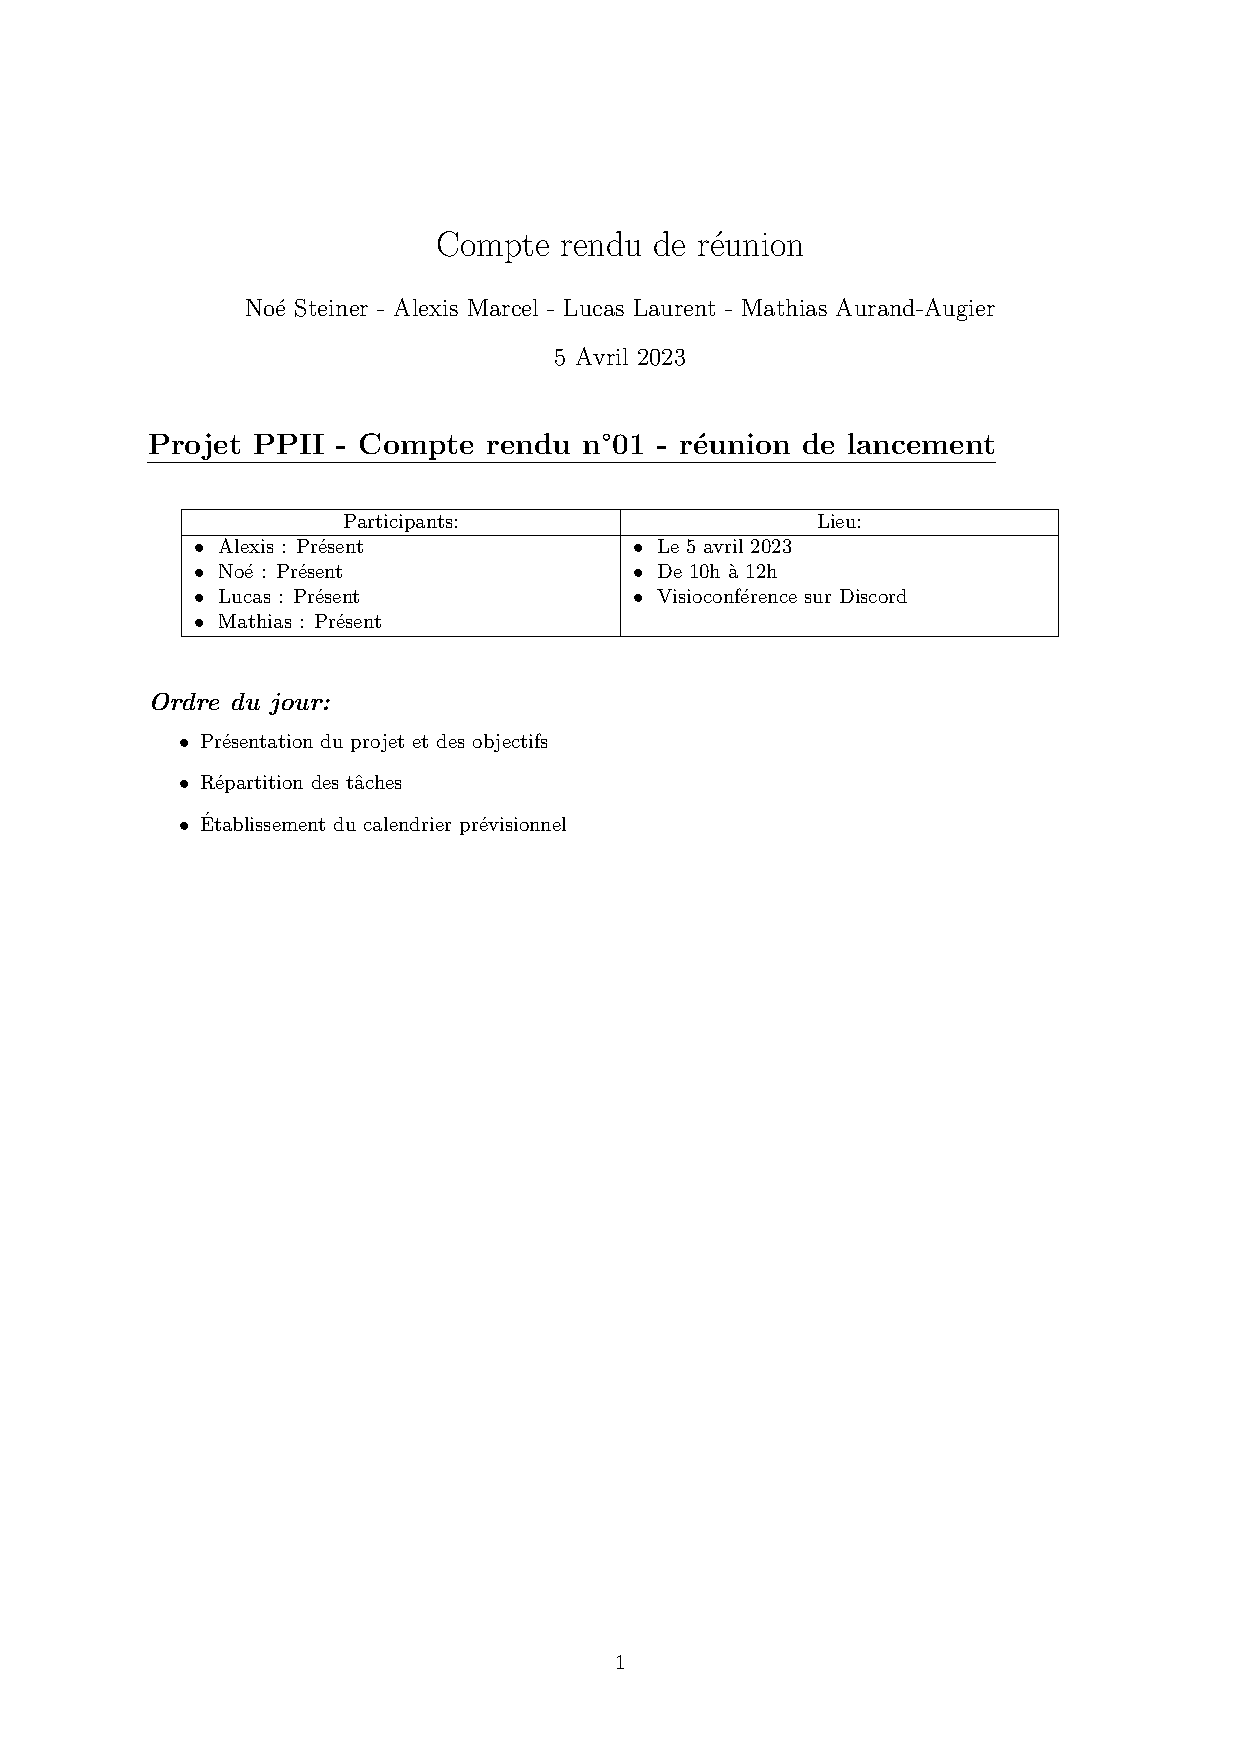
\includepdf[pages=1]{../cr_reu/reu1/cr_reu1.pdf}
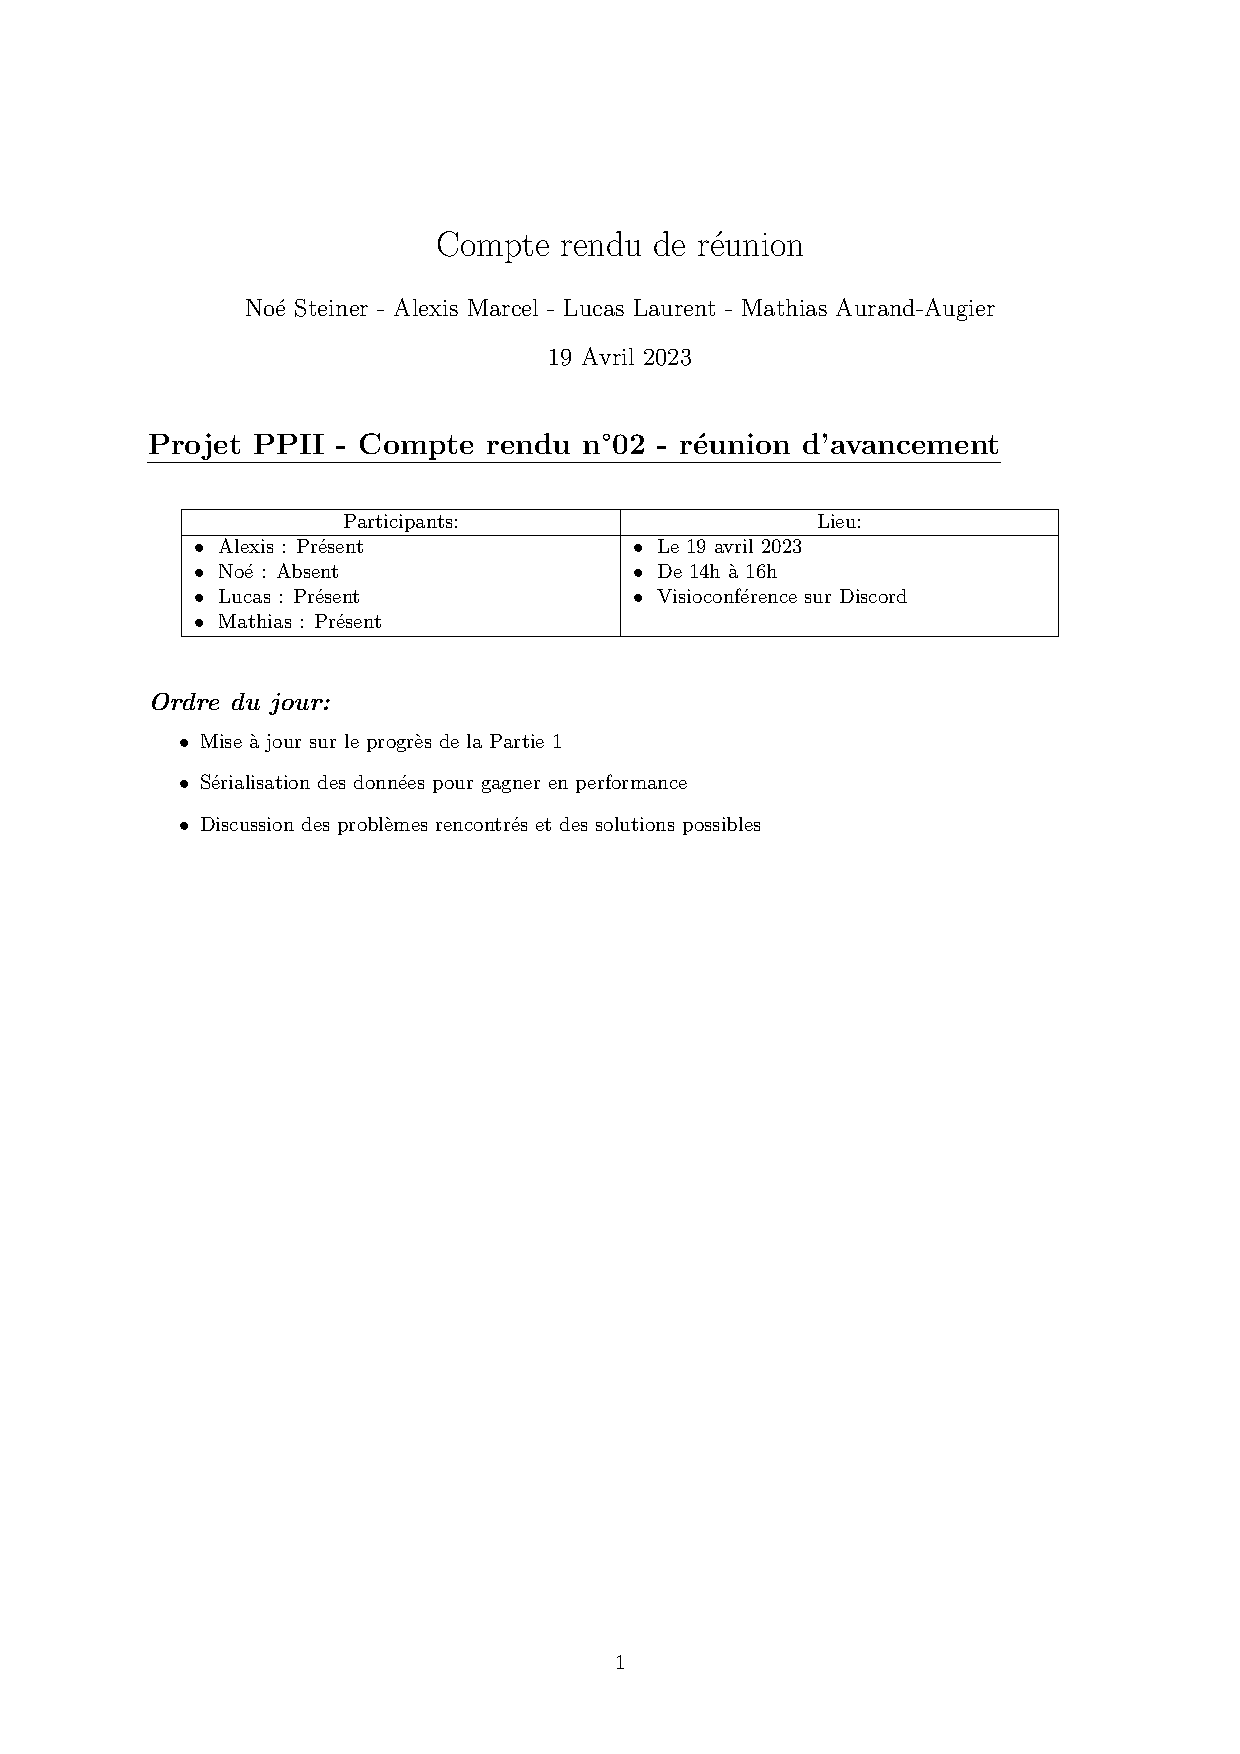
\includepdf[pages=1]{../cr_reu/reu2/cr_reu2.pdf}
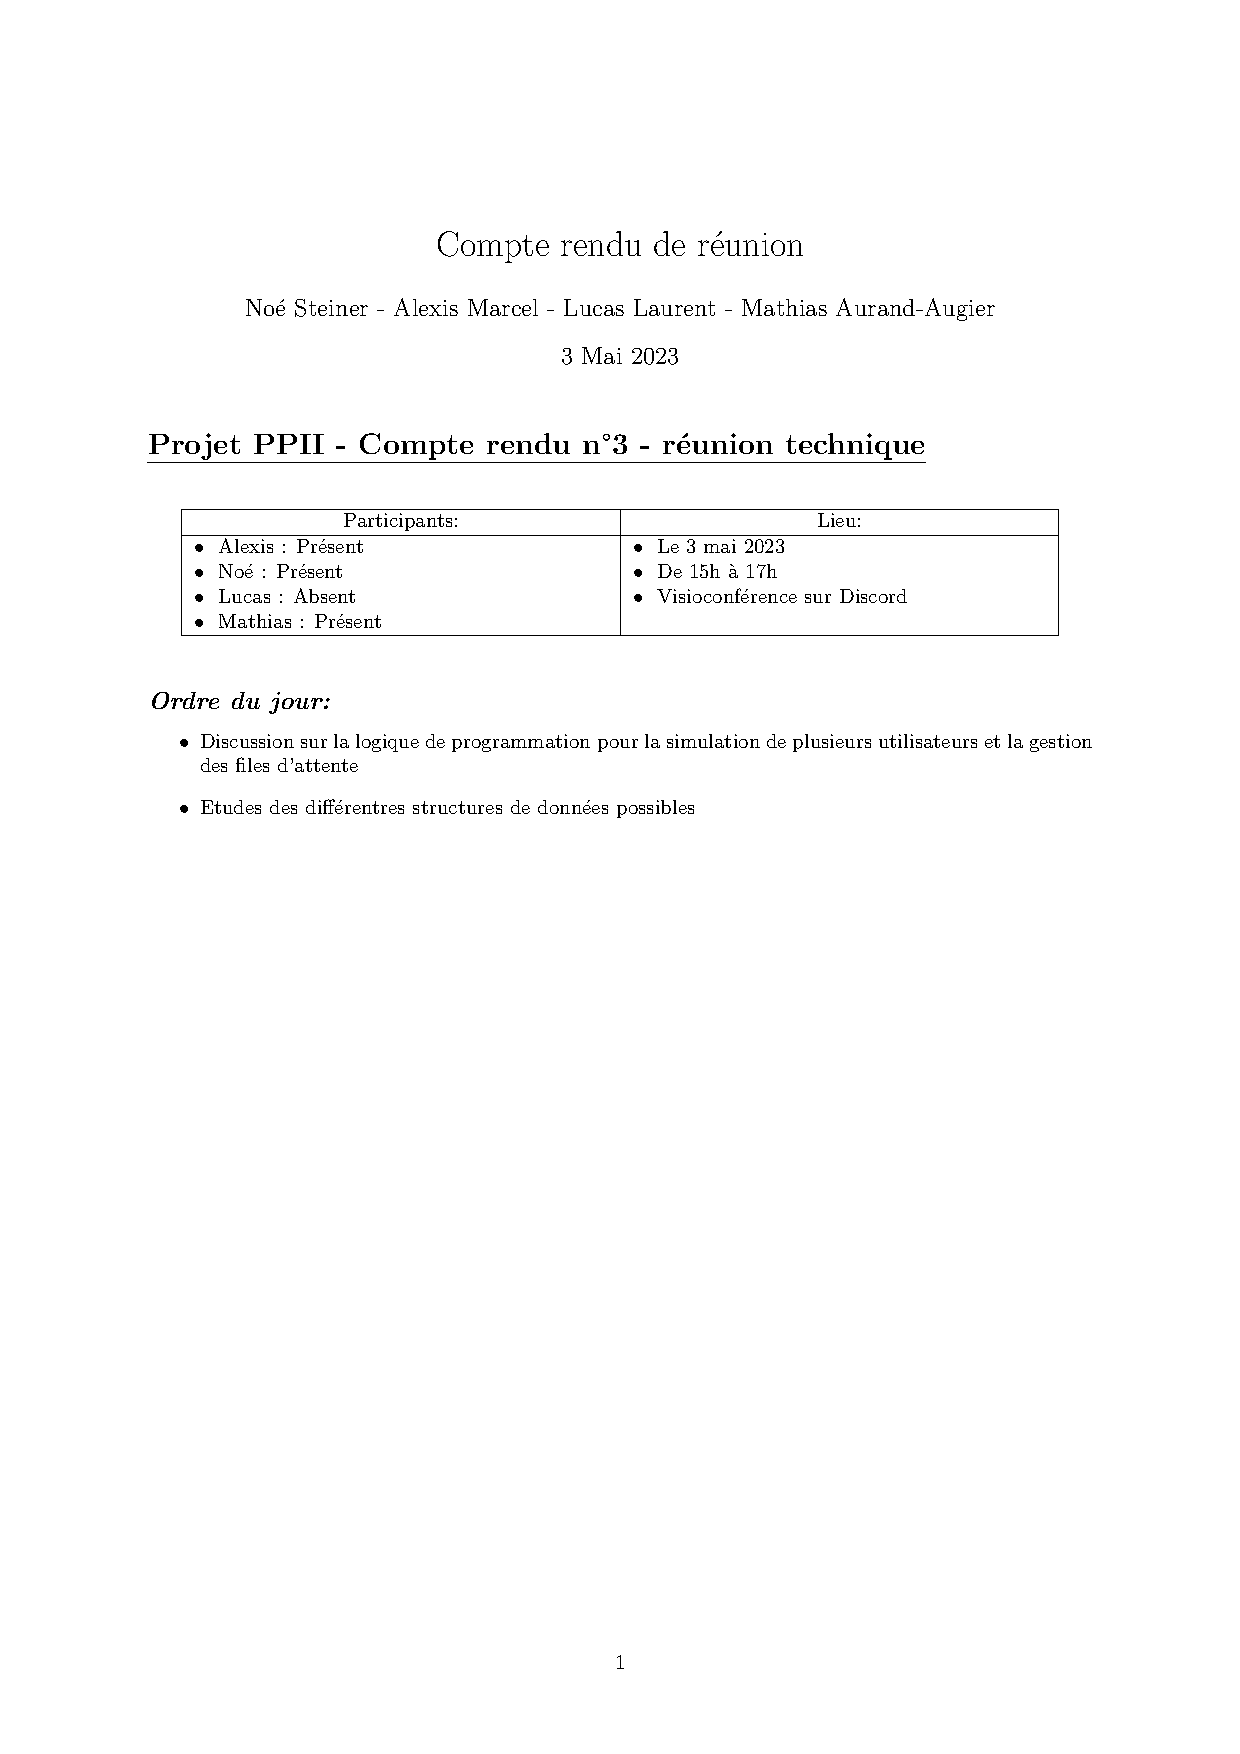
\includepdf[pages=1]{../cr_reu/reu3/cr_reu3.pdf}
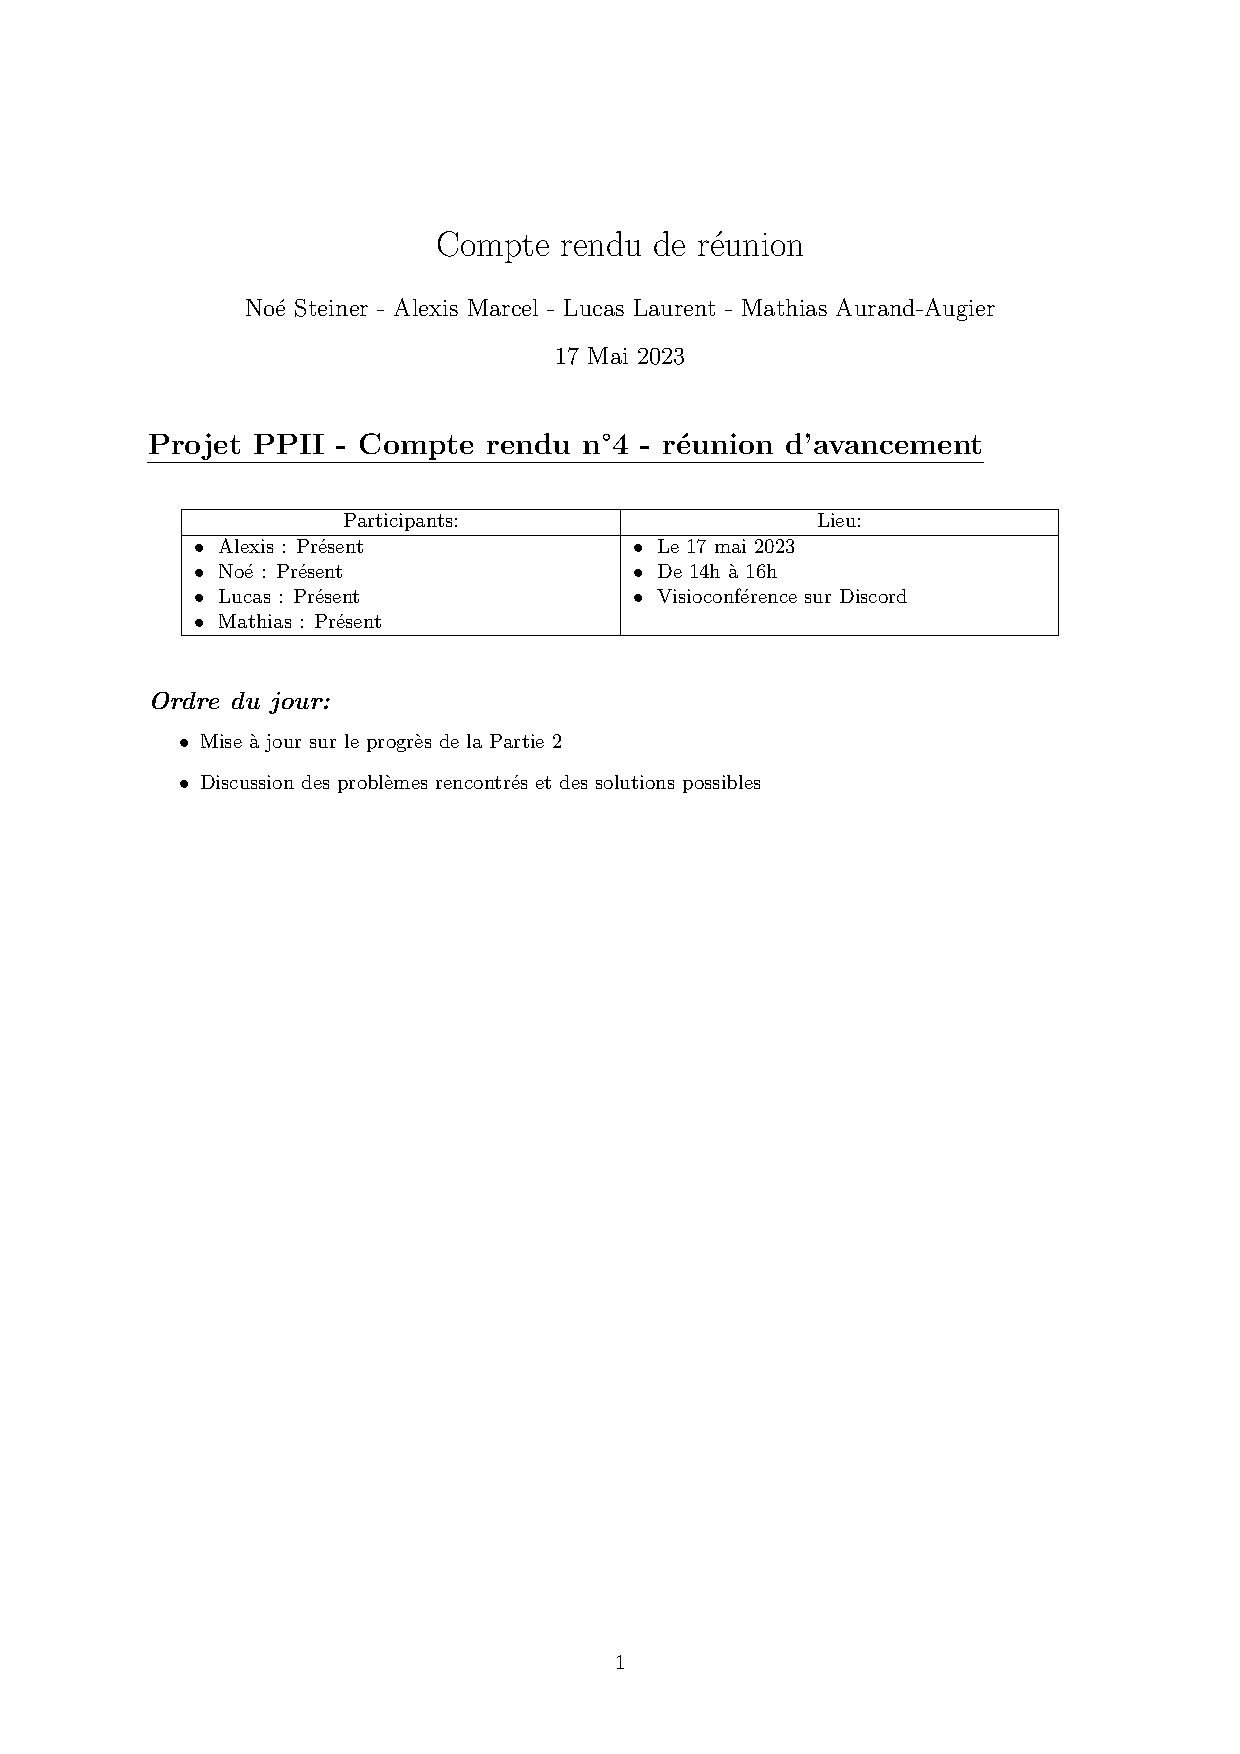
\includepdf[pages=1]{../cr_reu/reu4/cr_reu4.pdf}
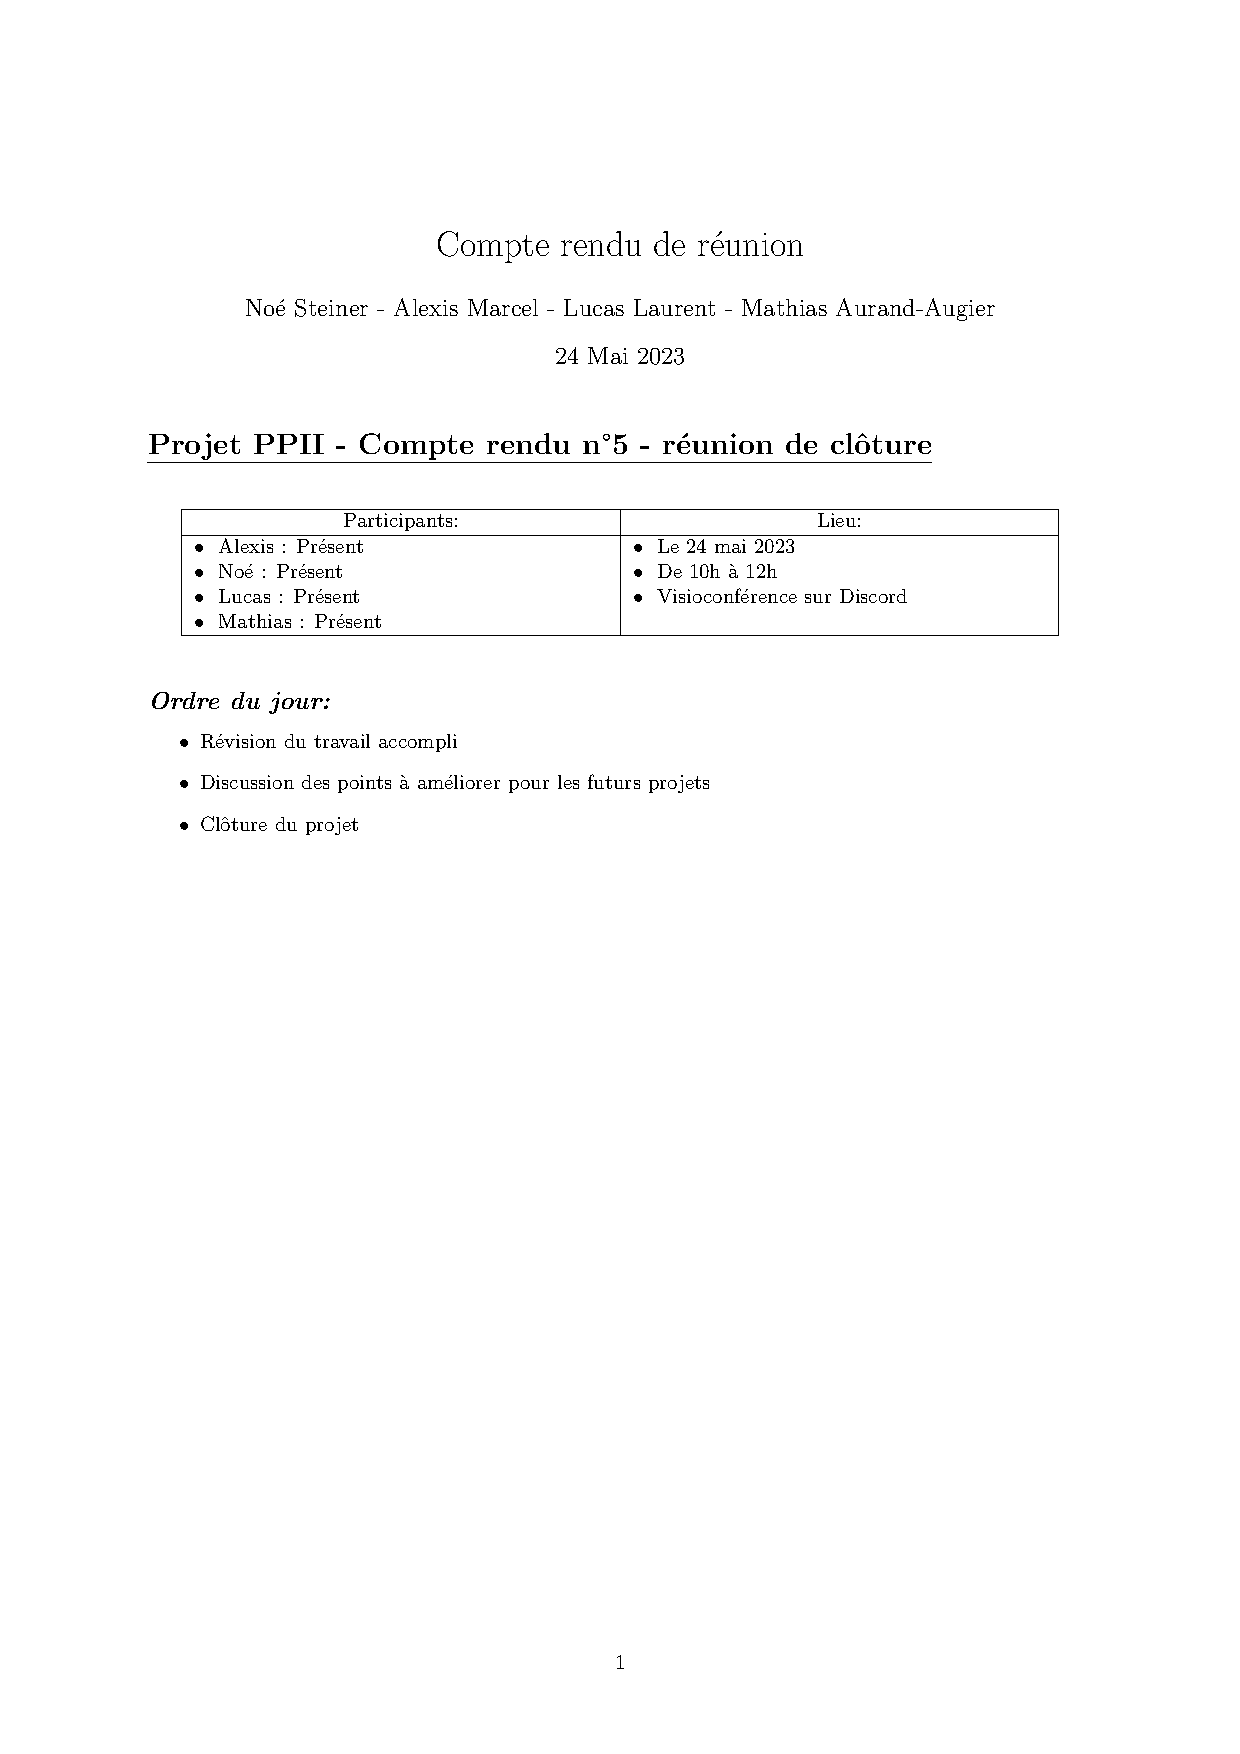
\includepdf[pages=1]{../cr_reu/reu5/cr_reu5.pdf}
\end{document}